\chapter{روش پیشنهادی}

\section{استراتژی تخلیه تصادفی}
با استفاده از مدل‌های توصیف شده در بخش‌های قبل، حال می‌توانیم یک تعریف ریاضی از «استراتژی تخلیه تصادفی» داشته باشیم. مشابه با مقاله \cite{Liu} یک استراتژی تخلیه تصادفی را به صورت توزیع احتمالی مانند \(g_\tau^a\) بر روی مجموعه \(S \times A\) تعریف می‌کنیم. در اینجا عبارت \(S \times A\) نمایانگر ضرب دکارتی مجموعه تمام حالت‌های سیستم در مجموعه تمام کنش‌های ممکن در سیستم است. یک نکته قابل توجه این است که برخی از دو تایی‌های حاصل از این ضرب دکارتی هیچ گاه در واقعیت امکان‌پذیر نیست. برای مثال در حالتی که صف خالی باشد تنها یک کنش امکان پذیر است و آن هم کنش شماره ۱ (\lr{No Operation}) است. با این حال برای سادگی در توضیح تئوری روش حل مسئله، این دو تایی‌ها را نیز در دامنه تابع توزیع احتمالی استراتژی تخلیه در نظر می‌گیریم تا همواره اندازه دامنه تابع احتمال برابر با مقدار ثابت \(|S| \cdot |A|\) باشد اما در پیاده‌سازی عملی چنین دوتایی‌هایی از دامنه حذف می‌شوند و مقدار احتمال ثابتی برابر صفر می‌گیرند تا با کاهش فضای حالت مسئله، سرعت الگوریتم اجرایی بهبود یابد. \\

همچنین طبق تعریف توزیع احتمال، رابطه \ref{eq:prob} باید برای هر استراتژی تخلیه تصادفی برقرار باشد.
\begin{equation}
	\label{eq:prob}
	\sum_{\tau \in S} \sum_{a \in A} g_{\tau}^{a}=1
\end{equation}
\section{مدل زنجیره مارکوف دستگاه کاربر}
در این قسمت ابتدا مدل آماری زنجیره مارکوف گسسته-زمان را معرفی می‌کنیم و سپس توضیح می‌دهیم که چگونه می‌توان با استفاده از این مدل معیارهای تاخیر و توان میانگین را برای یک سیستم تخلیه وظیفه محاسبه کرد.
\begin{defi}
\label{def:one}
دنباله‌ای از متغیرهای تصادفی $X_{1}, X_{2}, \ldots$ را که احتمال تغییر وضعیت از زمان $t$ به $t + 1$ مستقل از وضعیت‌های قبلی باشد را یک \textbf{زنجیره مارکوف گسسته-زمان} می‌نامند. این گزاره را به بیان متغیرهای تصادفی و تابع احتمال به صورت رابطه زیر نشان می‌دهیم.
\begin{equation*}
	\operatorname{Pr}\left(X_{t+1}=x \mid X_{1}=x_{1}, X_{2}=x_{2}, \ldots, X_{n}=x_{t}\right)=\operatorname{Pr}\left(X_{t+1}=x \mid X_{t}=x_{t}\right)
\end{equation*}
\end{defi}
زنجیره مارکوف گسسته‌-زمان را می‌توان با گراف جهت‌دار نیز نمایش داد. در شکل \ref{fig:gambler} یک زنجیره نمونه مشاهده می‌شود.
\begin{figure}[H]
	\centering
	\begin{latin}
			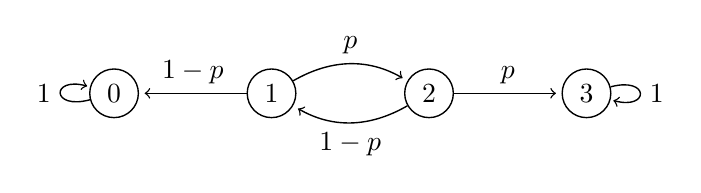
\begin{tikzpicture}[ - > , shorten >=2pt , line width =0.5 pt , node distance =2 cm]
			\node [circle , draw] (zero) {0};
			\node [circle , draw] (one) [right of=zero] {1};
			\node [circle , draw] (two) [right of=one] {2};
			\node [circle , draw] (three) [right of=two] {3};
			\path (zero) edge [loop left] node {$1$} (zero) ;
			\path (one) edge node [above] {$1 - p$} (zero) ;
			\path (one) edge [bend left] node [above]{$p$} (two) ;
			\path (two) edge node [above]{$p$} (three) ;
			\path (two) edge [bend left] node [below]{$1 - p$} (one) ;
			\path (three) edge [loop right] node {$1$} (three) ;
		\end{tikzpicture}
	\end{latin}
	\caption[یک مارکوف نمونه برای مسئله پاکباختگی]{یک زنجیره مارکوف نمونه برای مسئله پاکباختگی قمارباز\protect\footnotemark}
	\label{fig:gambler}
\end{figure}
\LTRfootnotetext{The Gambler's ruin}
\newpage
\begin{defi}
\label{def:two}
زنجیره مارکوف گسسته زمان $X(t)$ را \textbf{همگن-زمان} می‌گوییم اگر شرط زیر همواره برقرار باشد:
\begin{equation*}
P\left(X_{n+1}=j \mid X_{n}=i\right)=P\left(X_{1}=j \mid X_{0}=i\right)
\end{equation*}
به عبارت دیگر یعنی احتمالات مربوط به انتقال بین حالت‌ها به زمان \(t\) وابسته نیستند. در این حالت احتمال انتقال زنجیره از حالت \(i\) به \(j\) را با عبارت $p_{i j}=P\left(X_{1}=j \mid X_{0}=i\right)$ نمایش می‌دهیم و همچنین ماتریس انتقال را با $P=\left(p_{i j}\right)$ نمایش می‌دهیم. ماتریس انتقال را می‌توان به صورت یک گراف جهت‌دار نیز توصیف کرد به طوری که درایه $p_{i, j}$ در ماتریس معادل یک یال جهت‌دار از راس $i$ به راس $j$ با وزن $p_{i, j}$ است.
\end{defi}
طبق تعاریف \ref{def:one} و \ref{def:two} می‌توان زنجیره مارکوف گسسته‌زمانی برای حالت دستگاه کاربر در طی زمان در نظر گرفت که در آن حالت دستگاه کاربر $\tau[t]$ حالت زنجیره در زمان $t$ را مشخص می‌کند. همچنین ماتریس انتقال $\chi$ تعریف می‌شود به طوری که $\chi_{\tau, \tau^{\prime}}$ احتمال انتقال از حالت $\tau$ به \(\tau^{\prime}\) را مشخص می‌کند. \\

ماتریس انتقال را می‌توان به ازای یک استراتژی تخلیه داده شده و پارامترهای سیستمی مانند \(\alpha_1, \cdots, \alpha_k\) بدست آورد. در شکل \ref{fig:digraph} گراف جهت‌دار معادل زنجیره مارکوف برای یک سیستم با یک صف وظیفه و \(Q = 2\) و تعداد ۲ قسمت به ازای هر وظیفه و تعداد ۱ بسته به ازای هر وظیفه رسم شده است.\footnote{کد استفاده شده برای رسم این گراف در آدرس \lr{https://github.com/dalisyron/OffloadingVisualizer} موجود می‌باشد}
\begin{figure}[H]
\centering
\includegraphics[width=\textwidth]{figures/graph.pdf}
\caption[زنجیره مارکوف سیستم تخلیه در قالب گراف جهت دار]{
زنجیره مارکوف سیستم تخلیه در قالب گراف جهت دار (برای مشاهده جزئیات زوم کنید)
}
\label{fig:digraph}
\end{figure}
به منظور محاسبه معیارهایی مانند توان مصرفی میانگین و تاخیر سرویس میانگین لازم است که بتوانیم درباره وضعیت سیستم تخلیه وظیفه در طولانی‌مدت استنتاج کنیم. در همین راستا مفهوم توزیع پایدار را تعریف می‌کنیم.
\begin{defi}
به ازای یک زنجیره مارکوف داده شده با ماتریس انتقال \(P\) یک \textbf{توزیع پایدار} توزیع احتمالی مانند \(\pi\) است که شرط زیر برای آن برقرار باشد:
\begin{equation*}
	\pi=\pi P \quad \Longleftrightarrow \quad \pi_{j}=\sum_{i} \pi_{i} P_{i j} \quad \forall j .
\end{equation*}
\end{defi}
یک سوالی که ممکن است بوجود بیاید این است که آیا لزوما هر زنجیره مارکوف گسسته زمانی توزیع پایدار دارد؟ برای پاسخ به این سوال لازم است دو مفهوم زنجیره مارکوف تقلیل‌ناپذیر و غیرمتناوب را تعریف کنیم.
\begin{defi}
اگر رسیدن از هر نقطه به نقطه دیگر از فضای حالت با احتمال مثبت در زنجیره مارکوف میسر باشد، زنجیره را \textbf{تقلیل‌ناپذیر} گویند. به بیان ریاضی می‌توان تقلیل‌ناپذیر بودن زنجیره مارکوف را به صورت زیر نشان داد.
\begin{equation*}
	\operatorname{Pr}\left(X_{n_{i j}}=j \mid X_{0}=i\right)=p_{i j}^{\left(n_{i j}\right)}>0
\end{equation*}
\end{defi}

\begin{defi}
تناوب $d(i)$ برای حالت $i$ به صورت $d(i)=\operatorname{gcd}\left\{n: P_{i i}^{n}>0\right\}$ تعریف می‌شود، که به معنی بزرگ‌ترین مقسوم علیه مشترک تعداد مراحل ممکن است به صورتی که از $i$ شروع کرده و به $i$ برگردیم. یک زنجیره مارکوف تقلیل‌ناپذیر را متناوب با تناوب $d$ می‌گوییم اگر تمامی حالت‌ها تناوب $d > 1$ را داشته باشند. یک زنجیره مارکوف تقلیل ناپذیر را \textbf{غیرمتناوب} می‌گوییم اگر تمامی حالت‌ها تناوب برابر ۱ داشته باشند.
\end{defi}
\begin{thm}
\textbf{(همگرایی)}
هر زنجیره مارکوف تقلیل‌ناپذیر و غیر متناوب دارای توزیع پایدار منحصر به فردی مانند $\pi$ می‌باشد.
\end{thm}
حال با استفاده از قضیه ۳.۱. ثابت می‌کنیم که زنجیره مارکوف مربوط به سیستم تخلیه وظیفه دارای توزیع پایدار منحصر به فرد است. برای سادگی فرض می‌کنیم که سامانه یک صف دارد و سپس نحوه بسط نتیجه به چندین صف را توضیح می‌دهیم.

\begin{thm}
\label{thm:irreducible}
زنجیره مارکوف مربوط به سیستم تخلیه تک صف تقلیل ناپذیر است. \\
\textbf{اثبات:} \\
قسمت الف) با توجه به تعریف سیستم تخلیه می‌دانیم که از هر حالت غیر شروع مانند \( (0, 0, 0) \neq (x, y, z)\) می‌توان به حالت شروع رفت. به این منظور کافی است که تمام وظایف داخل صف به نحوی (اجرا یا ارسال) به اتمام برسند و وظیفه جدیدی نیز در این حین وارد سیستم نشود. \\

قسمت ب) همچنین می‌توان ثابت کرد که از حالت شروع \((0, 0, 0)\) می‌توان به هر حالت دیگر \((x, y, z)\) رفت. به این منظور دنباله رخدادهای زیر را در نظر بگیرید:
\begin{enumerate}
	\item ورود \(x\) وظیفه جدید
	\item انتقال یک وظیفه به واحد ارسال و ورود یک وظیفه جدید، هر دو در صورتی که \(y > 0\)
	\item پیشرفت واحد ارسال به مدت \(y\) سیکل و عدم ورود وظیفه جدید در این حین
	\item انتقال یک وظیفه به پردازنده و ورود یک وظیفه جدید، هر دو در صورتی که \(z > 0\)
	\item پیشرفت واحد ارسال به مدت \(z\) سیکل و عدم ورود وظیفه جدید در این حین
\end{enumerate}
با توجه به نتایج بخش الف و ب می‌توان نتیجه گرفت که از گشتی با احتمال مثبت از هر حالت به حالت دیگر وجود دارد بنابراین طبق تعریف زنجیره تقلیل‌ناپذیر است.
\end{thm}
\begin{thm}
\label{thm:aperiodic}
زنجیره مارکوف مربوط به سیستم تخلیه تک صف غیر متناوب است. \\
\textbf{اثبات:} \\
به منظور اثبات این قضیه فقط کافی است که به این نکته توجه کنیم که در زنجیره حالت \((0, 0, 0)\) دارای تناوب یک می‌باشد. زیرا با احتمالی مثبت (متناظر با رخداد عدم ورود وظیفه و کنش \lr{No Operation}) می‌توان در همان حالت ماند. با توجه به همین نکته و تقلیل‌ناپذیر بودن زنجیره میتوانیم نتیجه بگیریم که سایر حالت‌ها نیز باید تناوب یک داشته باشند. بنابراین زنجیره غیرمتناوب است.
\end{thm}
با توجه به قضایای \ref{thm:irreducible} و \ref{thm:aperiodic} و قضیه همگرایی می‌توان نتیجه گرفت که زنجیره مارکوف سیستم تخلیه تک صف دارای توزیع پایدار منحصر به فرد می‌ مطابق با رابطه \ref{eq:steady} می‌باشد. برای بسط این اثبات به حالت چند صف اثبات غیرمتناوب بودن یکسان خواهد بود و در اثبات تقلیل‌ناپذیر بودن، رخداد اول به ورود \(x_1, \cdots, x_k\) وظیفه از انواع مختلف تغییر پیدا می‌کند.
\begin{equation}
	\label{eq:steady}
	\left\{\begin{array}{l}
		\sum_{\boldsymbol{\tau}^{\prime} \in \mathcal{S}} \chi_{\boldsymbol{\tau}^{\prime}, \boldsymbol{\tau}} \pi_{\boldsymbol{\tau}^{\prime}}=\pi_{\boldsymbol{\tau}}, \forall \boldsymbol{\tau} \in \mathcal{S} \\
		\sum_{\boldsymbol{\tau} \in \mathcal{S}} \pi_{\boldsymbol{\tau}}=1
	\end{array}\right.
\end{equation}
\section{محاسبه تاخیر میانگین}
تاخیر هر وظیفه شامل تاخیر انتظار در صف وظایف و تاخیر پردازش می‌باشد. به منظور بدست آوردن تاخیر میانگین سیستم ابتدا $\theta_i$ را به عنوان کسری از وظایف سیستم در طولانی مدت که از نوع $i$ هستند تعریف می‌کنیم. اگر طول صف‌ها به مقدار کافی بزرگ باشد و همچنین استراتژی تخلیه‌ای داشته باشیم که منجر به پر شدن صف و اتلاف وظیفه\LTRfootnote{Task Loss} نشود مقدار $\theta_i$ طبق رابطه \ref{eq:theta} بدست می‌آید.
\begin{equation}
\label{eq:theta}
\theta_i = \frac{\alpha_i}{\sum_{j=1}^{k} \alpha_{j}}
\end{equation}
\newpage
پارامتر \(t_q^i\) را برابر با مقدار میانگین تاخیر انتظار در صف مربوط به وظایف نوع $i$ تعریف می‌کنیم. طبق قانون \lr{Little} می‌توان مقدار این تاخیر را بر اساس رابطه \ref{eq:queuing-delay} بدست آورد. همانطور که پیش‌تر ذکر شد برای برقراری این رابطه لازم است که اتلاف وظیفه در صف هیچ‌گاه رخ ندهد. به عبارت دیگر با فرض اینکه استراتژی تخلیه‌ی ارائه شده «کارامد» باشد این رابطه برقرار است. در پیاده‌سازی عملی، محدودیت «کارآمد» بودن یک استراتژی بدین گونه تعریف شده است که احتمال پر بودن صف حداکثر مقداری ناچیز  باشد.

\begin{equation}
	\label{eq:queuing-delay}
	t_{q}^i=\frac{\theta_i}{\alpha_i} \sum_{j=0}^{Q} i \cdot \operatorname{Pr}\{q_i[t]=i\}=\frac{1}{\alpha} \sum_{\tau \in S} \tau\{q_i\} \cdot \pi_{\tau}
\end{equation}
همچنین $t_{tx}^i$ را به عنوان تاخیر ارسال میانگین یک وظیفه از نوع \(i\) توسط واحد ارسال تعریف می‌کنیم که مقدار آن بر اساس امید ریاضی موفقیت در فرآیند برنولی مطابق با رابطه \ref{eq:bernouli} بدست می‌آید.
\begin{equation}
	\label{eq:bernouli}
	t_{t x}^i=M_i \sum_{j=1}^{\infty} j(1-\beta)^{(j-1)} \beta
\end{equation}
به یاد داریم که مقدار تاخیر در صورت پردازش محلی برای وظایف نوع $i$ برابر $L_i$ می‌باشد. تاخیر اجرا در صورت تخلیه وظیفه به صورت مجموع زمان ارسال وظیفه
$t_{tx}^i$
زمان اجرا در سرور لبه‌ای
$C_i$
و تاخیر دریافت نتیجه از سرور
$t_{rx}^i$
محاسبه می‌شود.
\begin{equation}
	t_{c}^i=t_{t x}^i+C_i+t_{rx}
\end{equation}
در نتیجه می‌توان تاخیر اجرای میانگین وظایف نوع $i$ را نیز مطابق رابطه \ref{eq:proc-delay} بیان کرد.
\begin{equation}
	\label{eq:proc-delay}
	t_{p}^i=\eta_i L_i+(1-\eta_i) t_{c}^i
\end{equation}
که در آن
$\eta_i$
بیانگر کسری از وظایف نوع $i$ می‌باشد که در طولانی‌مدت به صورت محلی اجرا می‌شوند و مطابق با رابطه \ref{eq:eta} بدست می‌آيد.
\begin{equation}
	\label{eq:eta}
	\eta_i=\frac{\sum_{\boldsymbol{\tau, a} \in \mathcal{S}_{1}^i\cup\mathcal{S}_{3}^i\cup\mathcal{S}_{5}^i} \pi_{\boldsymbol{\tau}} g_{\boldsymbol{\tau}}^{a} }{\sum_{\boldsymbol{\tau, a} \in \mathcal{S}_{1}^i\cup\mathcal{S}_{2}^i\cup\mathcal{S}_{3}^i\cup\mathcal{S}_{4}^i} \pi_{\boldsymbol{\tau}} g_{\boldsymbol{\tau}}^{a} + 2 \sum_{\boldsymbol{\tau, a} \in S_5^i} \pi_{\boldsymbol{\tau}} g_{\boldsymbol{\tau}}^{a}}
\end{equation}
که در آن
$S_1^i, \cdots, S_5^i$
به صورت زیر تعریف می‌شوند:
\begin{equation}
	\begin{aligned}
		& S_1^i = \{\boldsymbol{\tau, a} \in \mathcal{S} \times A | type(a) = AddToCPU \land locType(a) = i\} \\
		& S_2^i = \{\boldsymbol{\tau, a} \in \mathcal{S} \times A | type(a) = AddToTU \land offloadType(a) = i\} \\ 
		& S_3^i = \{\boldsymbol{\tau, a} \in \mathcal{S} \times A | type(a) = AddToBoth \land locType(a) = i \land offloadType(a) \neq i\} \\
		& S_4^i = \{\boldsymbol{\tau, a} \in \mathcal{S} \times A | type(a) = AddToBoth \land locType(a) \neq i \land offloadType(a) = i\} \\
		& S_5^i = \{\boldsymbol{\tau, a} \in \mathcal{S} \times A | type(a) = AddToBoth \land locType(a) = i \land offloadType(a) = i\}
	\end{aligned}
\end{equation}
در رابطه فوق تابع $type(a)$ نوع کنش را مشخص می‌کند و یکی از چهار نوع بیان شده در بخش \ref{sec:action} می‌باشد. توابع
$locType(a)$
و
$offloadType(a)$
نیز نوع وظیفه مربوط به کنش $a$ را مشخص می‌کنند. \\

با استفاده از روابط بالا همچنین می‌توانیم میانگین تاخیر سرویس هر وظیفه در سیستم را طبق رابطه \ref{eq:total-delay} محاسبه کنیم. نکته مهم این است که این تابع همان تابع هدف برای کمینه‌سازی در مسئله پیدا کردن استراتژی تخلیه بهینه است.
\begin{equation}
	\label{eq:total-delay}
	\bar{T}=\sum_{i=1}^{k} \theta_{i}\left(t_{q}^{i}+t_{p}^{i}\right)
\end{equation}
\newpage
\section{توان مصرفی میانگین}
اگر پارامتر
$\mu_\tau^{loc}$
و 
$\mu_\tau^{tx}$
را که به ترتیب به عنوان احتمال فعالیت پردازنده در حالت
$\tau$
و احتمال فعالیت واحد ارسال در حالت
$\tau$
تعریف کنیم، آنگاه توان مصرفی میانگین طبق رابطه زیر بدست می‌آید:
\begin{equation}
	\bar{P}=\sum_{\boldsymbol{\tau} \in \mathcal{S}} \pi_{\boldsymbol{\tau}}\left(\mu_{\boldsymbol{\tau}}^{l o c} P_{l o c}+\mu_{\boldsymbol{\tau}}^{t x} P_{t x}\right)
\end{equation}

\section{استراتژی تخلیه وظیفه بهینه}
\label{sec:strat}
با توجه به توابع بدست آمده برای تاخیر و توان مصرفی میانگین در بخش‌های پیشین، حال می‌توانیم مسئله پیدا کردن استراتژی تخلیه بهینه را به صورت یک مسئله بهینه سازی مانند
$\mathcal{P}_{1}$
بیان کنیم:
\begin{equation}
		\begin{aligned}
			\mathcal{P}_{1}: \min _{\left\{g_{\tau}^{a}\right\}}\; & \bar{T} = (\sum_{i=1}^{k} \frac{1}{\alpha_i} \sum_{\tau \in S} \tau\{q_i\} \cdot \pi_{\tau}) + T_p^0 \\
			\text { \lr{s.t.} } &\left\{\begin{array}{l}
				\bar{P} \leq \bar{P}_{\max } \\
				\sum_{\boldsymbol{\tau}^{\prime} \in \mathcal{S}} \chi_{\boldsymbol{\tau}^{\prime}, \boldsymbol{\tau}} \pi_{\boldsymbol{\tau}^{\prime}}=\pi_{\boldsymbol{\tau}}, \boldsymbol{\tau} \in \mathcal{S}, \\
				\sum_{\boldsymbol{\tau} \in S} \pi_{\boldsymbol{\tau}}=1, \\
				\sum_{\alpha \in A} g_{\tau}^{\alpha}=1, \forall \tau \in S\\
				g_{\tau}^{a} \geq 0, \forall \tau \in S,\;a \in A
			\end{array}\right.
		\end{aligned}
\end{equation}
که در آن
$T_p^0$
برابر با تاخیر اجرای میانگین است که به ازای مقادیر داده شده از
$\eta_0, \cdots, \eta_k$
مقداری ثابت دارد و از رابطه زیر بدست می‌آید:
\begin{equation}
	T_p^0 = \sum_{i=1}^{k} (\eta_i L_i+(1-\eta_i) t_{c}^i)
\end{equation}
\clearpage
با توجه به وجود پارامتر $\eta_i$ در تابع هدف
$\mathcal{P}_{1}$
این مسئله بهینه‌سازی، یک مسئله خطی نیست. با این حال می‌توانیم با استفاده از تغییری کوچک مسئله را به دنباله‌ای از مسائل برنامه‌ریزی خطی تبدیل کنیم. به این منظور مشابه \cite{Liu} از تعریف «معیار احاطه\LTRfootnote{Occupation Measure}» در زنجیره مارکوف استفاده می کنیم. به طور دقیق‌تر مجموعه متغیرهای جدید $\left\{x_{\tau}^{a}\right\}$ را تعریف می‌کنیم به طوری که  $x_{\tau}^{a}=\pi_{\tau} g_{\tau}^{a}$ تعریف می‌کنیم. به عبارتی $x_{\tau}^{a}$ برابر با احتمال حضور در حالت $\tau$ و انتخاب کنش
$a$
می‌باشد. همچنین طبق تعریف 
$\sum_{a \in A} g_{\tau}^{a}=1$
و بنابراین
$\pi_{\boldsymbol{\tau}}=\sum_{a \in A} x_{\boldsymbol{\tau}}^{a}$
\\\\
حال با جایگذاری $\left\{x_{\tau}^{a}\right\}$ به جای $\{\pi_\tau\}$ در
$\mathcal{P}_{1}$
خواهیم داشت:
\begin{equation}
	\label{eq:p2}
	\begin{aligned}
		\mathcal{P}_{2}: \min _{\boldsymbol{x}, \eta}\; & \bar{T}=(\sum_{i=1}^{k} \frac{1}{\alpha_i} \sum_{\tau \in \mathcal{S}} \sum_{a \in A} \tau\{q_i\} \cdot x_{\tau}^{a})+ T_p^0 \\
		\text { \lr{s.t.} } &\left\{\begin{array}{l}
			\nu_{l o c}(\boldsymbol{x}) P_{l o c}+\beta \nu_{t x}(\boldsymbol{x}) P_{t x} \leq \bar{P}_{\max } \\
			\Gamma(\boldsymbol{x}, \eta_i)=, \forall i \in \{1, \cdots, k\}\\
			F_{\tau}(\boldsymbol{x})=0, \forall \tau=(i, m, n) \in \mathcal{S} \\
			\sum_{\tau \in \mathcal{S}} \sum_{a \in A}=1 \\
			\eta_i \in [0, 1], \forall i \in \{1, \cdots, k\} \\
			x_{\tau}^{a} \geq 0, \forall \tau \in S, a \in A
		\end{array}\right.
	\end{aligned}
\end{equation}
که در آن
$\nu_{l o c}$
و
$\nu_{t x}$
به ترتیب احتمال فعالیت پردازنده و واحد ارسال را در یک واحد زمانی دلخواه مشخص می‌کنند و به ازای یک استراتژی داده شده قابل محاسبه اند. \footnote{برای مشاهده روش محاسبه این دو پارامتر در قالب کد به پیوست ۲ مراجعه شود.} تابع
$\Gamma(\boldsymbol{x}, \eta_i)$
بر اساس رابطه \ref{eq:eta} می‌باشد و به صورت زیر محاسبه می‌شود:
\begin{equation}
	\Gamma(x, \eta) = \eta  \sum_{\boldsymbol{\tau, a} \in \mathcal{S}_{1}^i\cup\mathcal{S}_{2}^i\cup\mathcal{S}_{3}^i\cup\mathcal{S}_{4}^i} x_{\tau}^a + 2 \eta \sum_{\boldsymbol{\tau, a} \in S_5^i} x_{\tau}^a
	- \eta \sum_{\boldsymbol{\tau, a} \in \mathcal{S}_{1}^i\cup\mathcal{S}_{3}^i\cup\mathcal{S}_{5}^i} x_{\tau}^a
\end{equation}
و تابع 
$F_{\tau}(\boldsymbol{x})$
به صورت زیر تعریف می‌شود:
\begin{equation}
	F_{\tau}(\boldsymbol{x})=\sum_{\tau^{\prime} \in \mathcal{S}} \sum_{a \in A} \tilde{\chi}_{\tau^{\prime}, \tau, a} x_{\tau^{\prime}}^{a}-\sum_{a \in A} x_{\tau}^{a}
\end{equation}
در رابطه فوق منظور از
$ \tilde{\chi}_{\tau^{\prime}, \tau, a}$
احتمال این است که به شرط اینکه در حالت
$\tau^{\prime}$
باشیم و کنش
$a$
انتخاب شده باشد، آنگاه به حالت
$\tau^{\prime}$
برویم. \\

در صورتی که مقادیر
$\eta_0, \cdots, \eta_k$
معلوم باشد آنگاه مسئله
$\mathcal{P}_2$
تبدیل به یک مسئله برنامه‌ریزی خطی می‌شود. با یافتن مقادیر جواب بهینه
$\left\{x_{\tau}^{a}\right\}$ 
می‌توان استراتژی بهینه را طبق رابطه زیر بدست آورد:
\begin{equation}
	g_{\tau}^{a *}=\frac{x_{\tau}^{a *}}{\sum_{a \in A} x_{\tau}^{a *}}, \forall \tau \in \mathcal{S}, a \in A
\end{equation}
بنابراین جهت یافتن استراتژی بهینه برای یک سیستم تخلیه وظیفه کافی است که مسئله برنامه‌ریزی خطی حاصل از
$\mathcal{P}_2$
را به ازای مقادیر مختلف 
$\eta_0, \cdots, \eta_k$
حل کرده تا استراتژی بهینه بدست بیاید. مراحل این فرآیند جستجو در الگوریتم ۱ به صورت خلاصه آمده است.

\begin{latin}
	\begin{algorithm}
		\rl{\caption{الگوریتم جستجوی استراتژی تخلیه وظیفه بهینه}\label{alg:cap}}
		\begin{algorithmic}[1]
			\Require $precision \geq 2$
			\State $etaSettings \gets splitRange([0, 1], precision)^k$
			\State $optimalPolicy = null$
		    \ForEach {$s \in etaSettings$}
				\State $(\eta_0, \cdots, \eta_k) \gets s$
				\State $solution \gets solveLP(\eta_0, \cdots, \eta_k)$
				\If{$optimalPolicy = null\;\mathbf{or}\;solution.delay < optimalPolicy.delay$}
					\State $optimalPolicy \gets solution.policy$
				\EndIf
			\EndFor \\
			\Return $optimalPolicy$
		\end{algorithmic}
	\end{algorithm}
\end{latin}